\documentclass[compress]{beamer}
\usepackage{ifthen,verbatim}

\title{New AlCa streams for CSC alignment}
\author{Jim Pivarski}
\institute{Texas A\&M University}
\date{28 February, 2008}

\newcommand{\isnote}{}
\xdefinecolor{lightyellow}{rgb}{1.,1.,0.25}
\xdefinecolor{darkblue}{rgb}{0.1,0.1,0.7}

%% Uncomment this to get annotations
%% \def\notes{\addtocounter{page}{-1}
%%            \renewcommand{\isnote}{*}
%% 	   \beamertemplateshadingbackground{lightyellow}{white}
%%            \begin{frame}
%%            \frametitle{Notes for the previous page (page \insertpagenumber)}
%%            \itemize}
%% \def\endnotes{\enditemize
%% 	      \end{frame}
%%               \beamertemplateshadingbackground{white}{white}
%%               \renewcommand{\isnote}{}}

%% Uncomment this to not get annotations
\def\notes{\comment}
\def\endnotes{\endcomment}

\setbeamertemplate{navigation symbols}{}
\setbeamertemplate{headline}{\mbox{ } \hfill
\begin{minipage}{5.5 cm}
\vspace{-0.75 cm} \small
\end{minipage} \hfill
\begin{minipage}{4.5 cm}
\vspace{-0.75 cm} \small
\begin{flushright}
\ifthenelse{\equal{\insertpagenumber}{1}}{}{Jim Pivarski \hspace{0.2 cm} \insertpagenumber\isnote/\pageref{numpages}}
\end{flushright}
\end{minipage}\mbox{\hspace{0.2 cm}}\includegraphics[height=1 cm]{../cmslogo} \hspace{0.1 cm} \includegraphics[height=1 cm]{../tamulogo} \hspace{0.01 cm} \vspace{-1.05 cm}}

\begin{document}
\frame{\titlepage}

%% \begin{notes}
%% \item This is the annotated version of my talk.
%% \item If you want the version that I am presenting, download the one
%% labeled ``slides'' on Indico (or just ignore these yellow pages).
%% \item The annotated version is provided for extra detail and a written
%% record of comments that I intend to make orally.
%% \item Yellow notes refer to the content on the {\it previous} page.
%% \item All other slides are identical for the two versions.
%% \end{notes}

%% \hspace{-0.83 cm} \textcolor{darkblue}{\Large Outline2}

\begin{frame}
\frametitle{Why?}

\begin{columns}
\column{0.7\linewidth}
\begin{itemize}\setlength{\itemsep}{0.1 cm}
\item CSC overlap regions could be very useful for relative alignment
of chambers on rings
\item Tracks don't propagate through iron between chambers, so the
energy threshold doesn't need to be as high
\item Procedure must reject non-overlap tracks, as they would
interfere with alignment
\item An enriched sample would make this more efficient
\item Collision muons and beam-halo muons are both good sources of
overlap tracks
\item Beam-halo is also useful in the non-overlap case, for layer
alignment
\end{itemize}

\column{0.3\linewidth}
\includegraphics[width=\linewidth]{overlap.png}
\end{columns}
\end{frame}

\begin{frame}
\frametitle{New streams}

There are cffs for three new streams in Alignment/CommonAlignmentProducer V00-26-00:

\vspace{0.1 cm}
\begin{itemize}\setlength{\itemsep}{0.25 cm}
\item \textcolor{darkblue}{ALCARECOMuAlOverlaps:} standard-trigger muons in an overlap region
\item \textcolor{darkblue}{ALCARECOMuAlBeamHalo:} beam-halo muons
\item \textcolor{darkblue}{ALCARECOMuAlBeamHaloOverlaps:} beam-halo muons in an overlap region
\end{itemize}

\vfill
Continuations of the new HLT paths presented at yesterday's Trigger Plenary.

\vfill
Two new track selector modules (analogous to AlignmentTrackSelectorModule):
\begin{itemize}
\item \textcolor{darkblue}{AlignmentCSCOverlapSelectorModule}
\item \textcolor{darkblue}{AlignmentCSCBeamHaloSelectorModule}
\end{itemize}
\end{frame}

\begin{frame}
\frametitle{\mbox{ }}

\vfill
\hspace{-0.83 cm} \textcolor{darkblue}{\Large Collision muons in the CSC overlap regions}

\vspace{0.5 cm}

\includegraphics[width=\linewidth]{path_standard.png}

\begin{itemize}\setlength{\itemsep}{0.25 cm}
\item Everything through ``standard reconstruction'' is just like
ALCARECOMuAlZMuMu, the standard muon alignment stream

\item AlignmentCSCOverlapSelectorModule selects tracks with $\ge$ 4 hits
on each of two chambers in the same station

\item Later in processing (during or before alignment procedure), the
same module will be used to select overlaps in a given station

\end{itemize}
\end{frame}

\begin{frame}
\frametitle{\mbox{ }}

\vfill
\hspace{-0.83 cm} \textcolor{darkblue}{\Large All CSC beam-halo}

\vspace{0.5 cm}
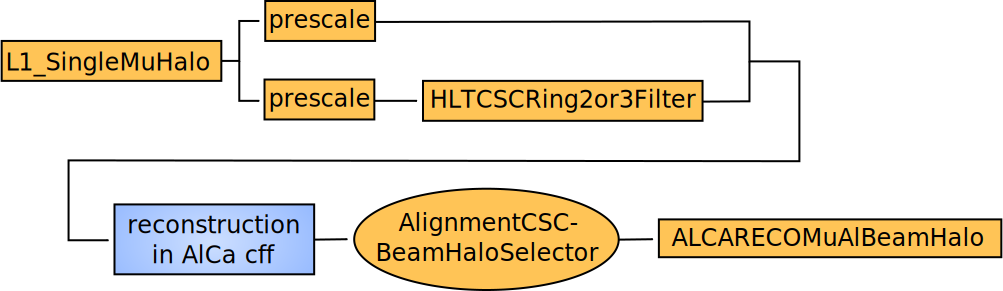
\includegraphics[height=2.4 cm]{path_beamhalo.png}

\begin{itemize}\setlength{\itemsep}{0.25 cm}
\item Beam-halo events need to be reconstructed with the non-standard CosmicMuonProducer

\item Proposal: do that reconstruction in the cff file that defines the AlCa stream

\item (same thing for tracker beam-gas and tracker cosmic rays)

\item AlignmentCSCBeamHaloSelectorModule requires $\ge$ 4 hits on a
given number of muon stations: the only way to cut on beam-halo energy
\end{itemize}
\end{frame}

\begin{frame}
\frametitle{\mbox{ }}

\hspace{-0.83 cm} \textcolor{darkblue}{\Large Beam-halo in the CSC overlap regions}

\vspace{0.5 cm}
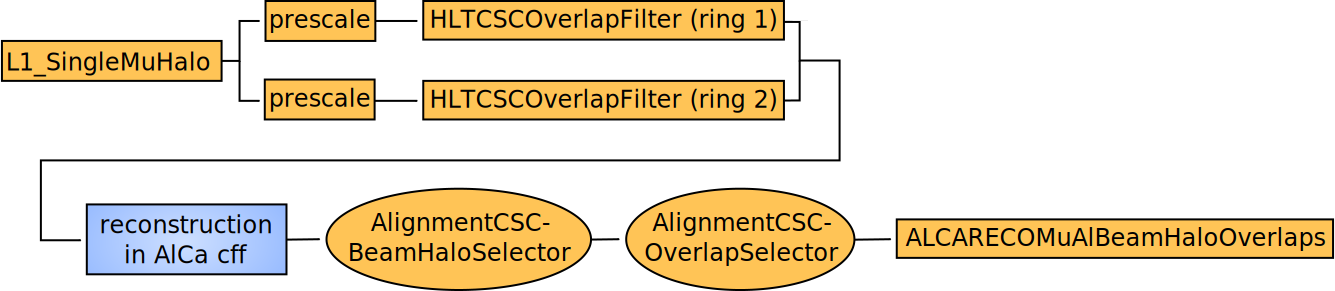
\includegraphics[height=2.4 cm]{path_beamhalo_overlap.png}

\begin{itemize}\setlength{\itemsep}{0.25 cm}
\item Re-use modules from the previous two cases

\item (the HLT paths are different)
\end{itemize}
\end{frame}

%% \section*{First section}
%% \begin{frame}
%% \begin{center}
%% \Huge \textcolor{blue}{First section}
%% \end{center}
%% \end{frame}

\begin{frame}
\frametitle{Conclusions}

Pending approval, I'd like these to be published to 2\_0\_X.

\vfill
\begin{itemize}\setlength{\itemsep}{0.35 cm}
\item The two selector modules have been tested on beam-halo MC.
\item The full AlCa chains have not: if there's a mistake, I'll need
to correct it before we attach these cffs to a real AlCa production
\item The L1 trigger bits at the beginning of the chain are not set to
meaningful values, anyway.
\end{itemize}

\label{numpages}
\end{frame}

\end{document}
